\section{Marco teórico}

    El presente proyecto tiene como objetivo principal un desarrollo tecnológico aplicado al campo del mantenimiento industrial. Lo anterior implica la combinación de varios conceptos que sirven como guía, tanto para el proceso de diseño como para la comprensión del alcance del mismo. A continuación, se presenta un esquema de la estructura conceptual sobre la cual se elaboró el marco teórico y, en consecuencia, se llevó a cabo el ya mencionado desarrollo tecnológico:

    \begin{figure}[H]
    \caption{Estructura conceptual del proyecto}
    \centering
    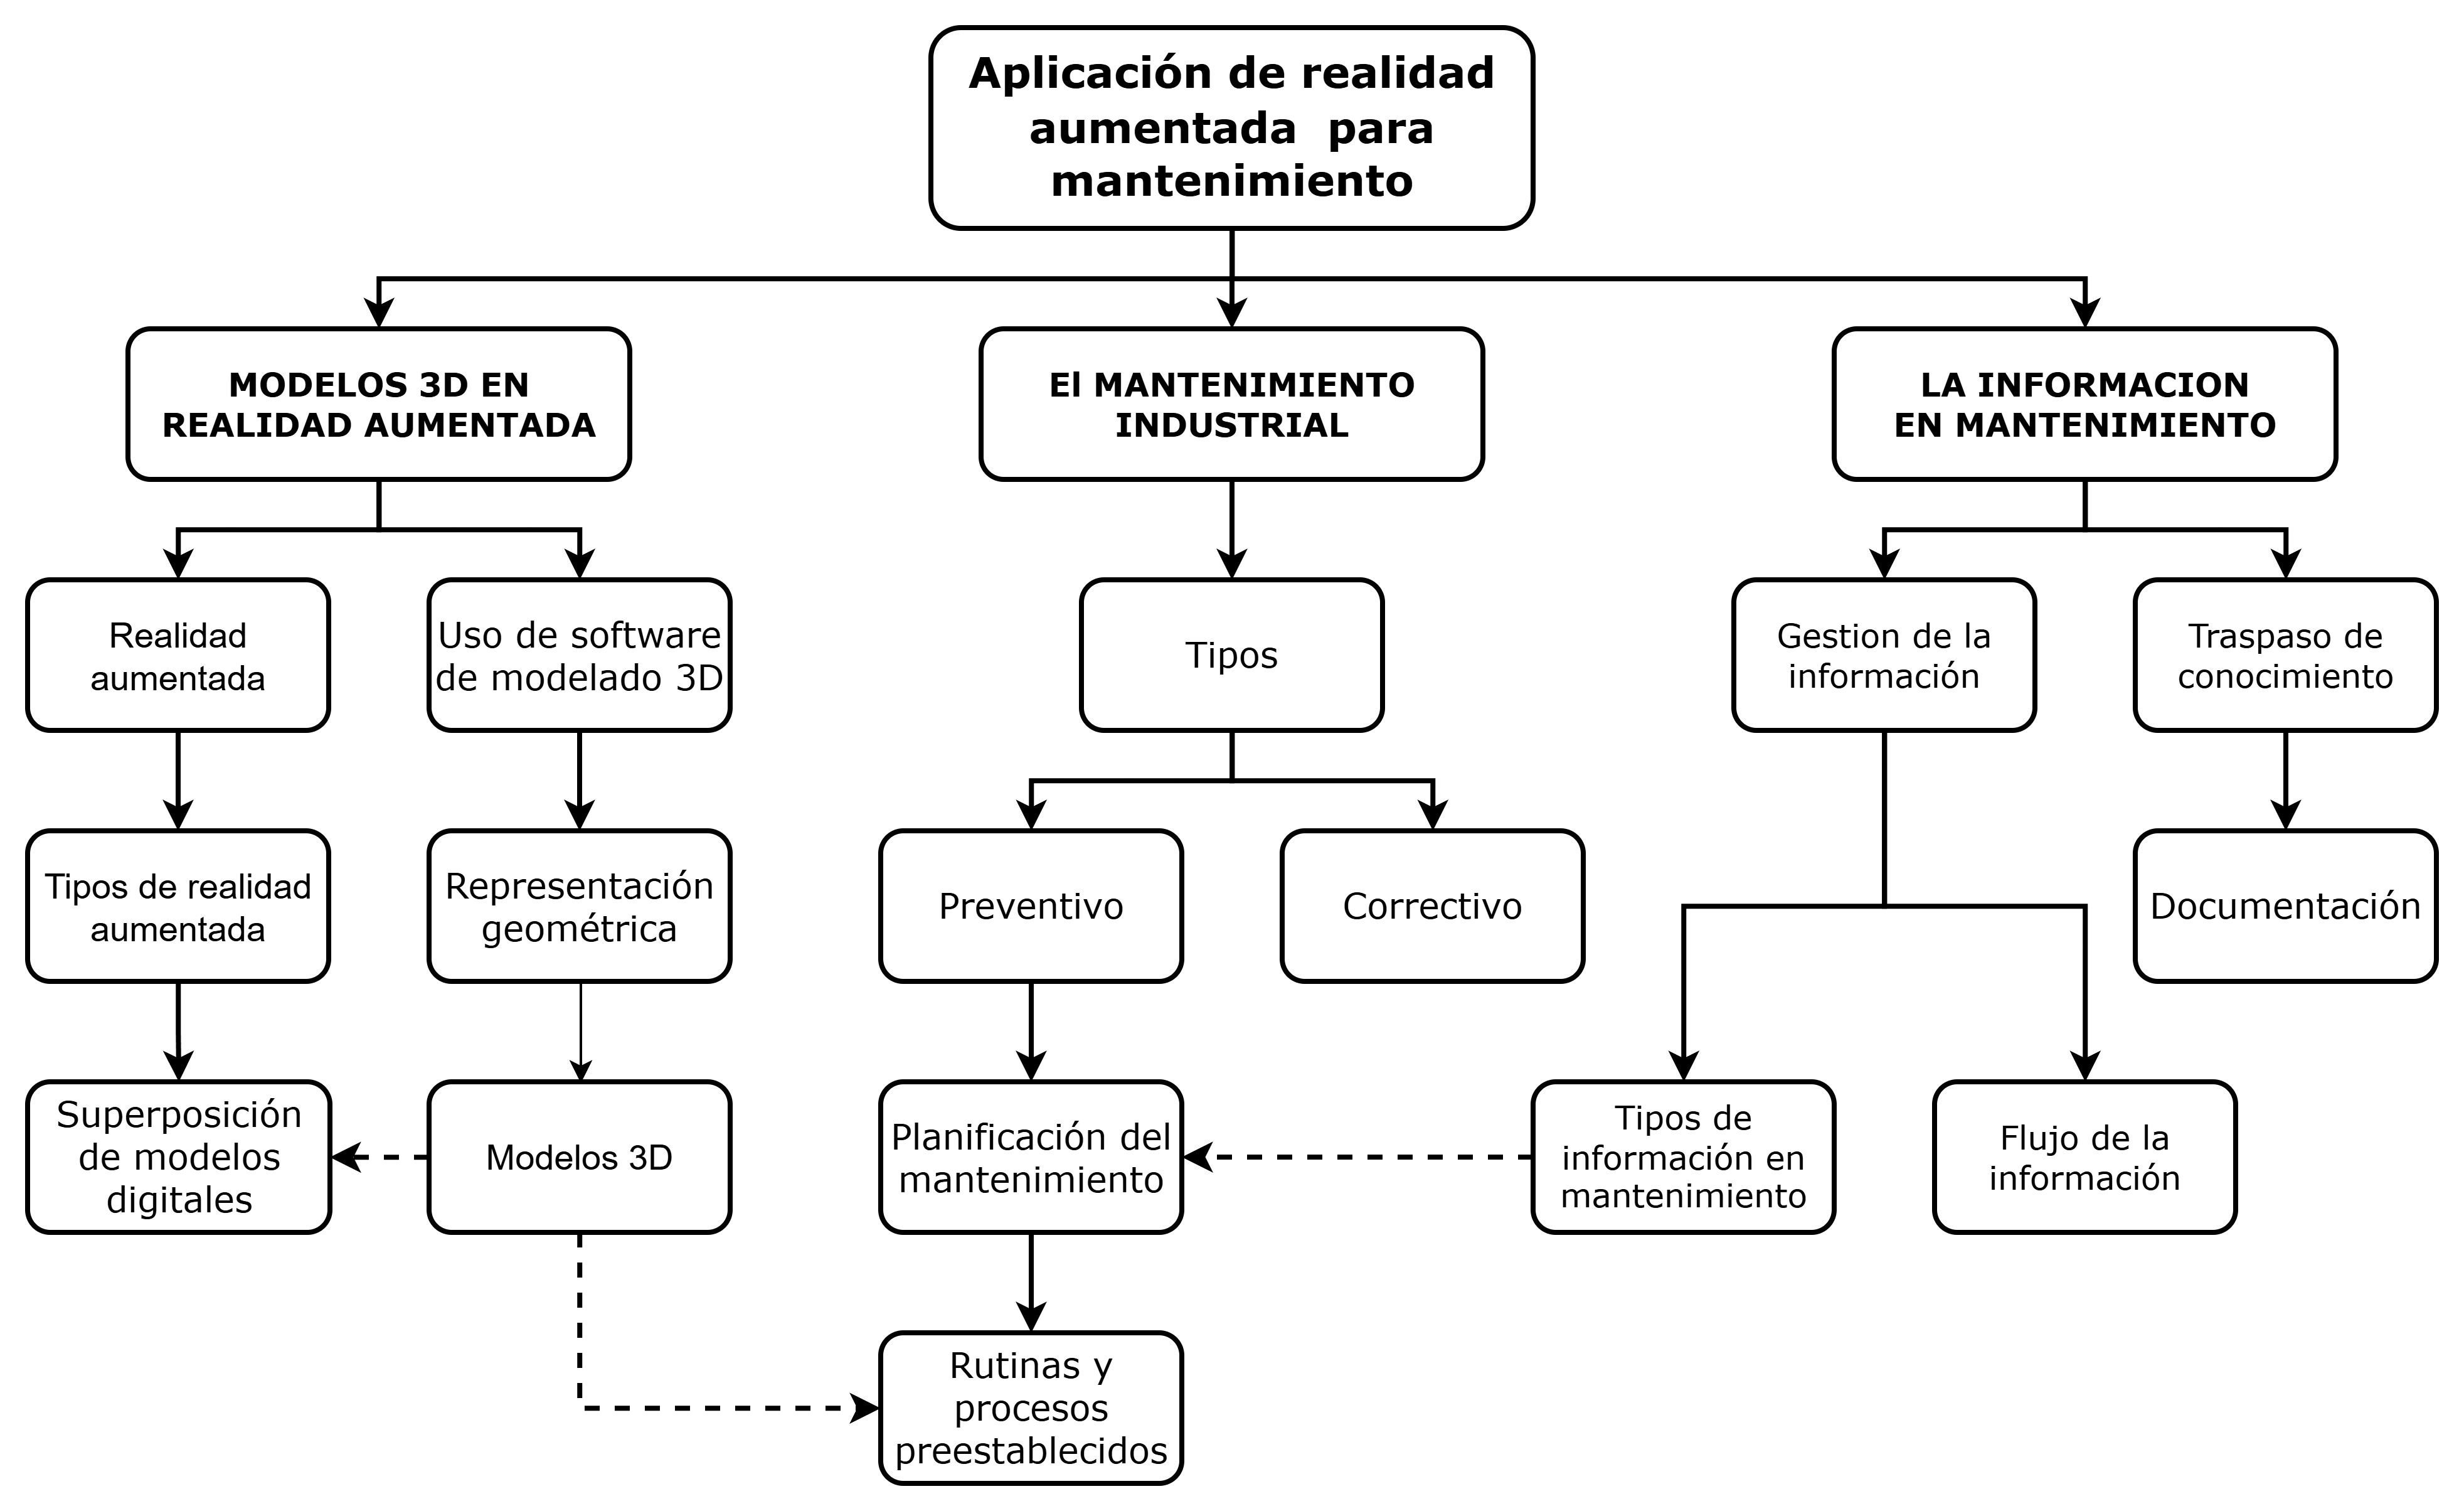
\includegraphics[width=\textwidth]{assets/figures/theoretical_framework/img_project_schema.png}
    \label{fig:mproject_schema}
\end{figure}
\fixvspace{1}

    \subsection{Mantenimiento industrial}

        El mantenimiento industrial constituye una función fundamental dentro de la gestión de los sistemas productivos de las empresas, ya que permite asegurar aspectos como la disponibilidad, confiabilidad y seguridad de los equipos e instalaciones a lo largo del tiempo. La normativa de la Unión Europea define al mantenimiento como la “combinación de todas las acciones técnicas, administrativas y de gestión realizadas durante el ciclo de vida de un elemento, destinadas a conservar o a devolverlo a un estado en el que pueda desempeñar la función requerida” \parencite{UNE:2018}.

        El mantenimiento se puede clasificar según si se actúa previa o posteriormente al evento de una falla de un equipo. En la Figura \ref{fig:maintenance_categories} se muestra el esquema de dicha clasificación, con los nombres con los que se conocen a estas formas de abordar las acciones de mantención:

        \begin{figure}[H]

    \caption{Categorías del mantenimiento}

    \centering
    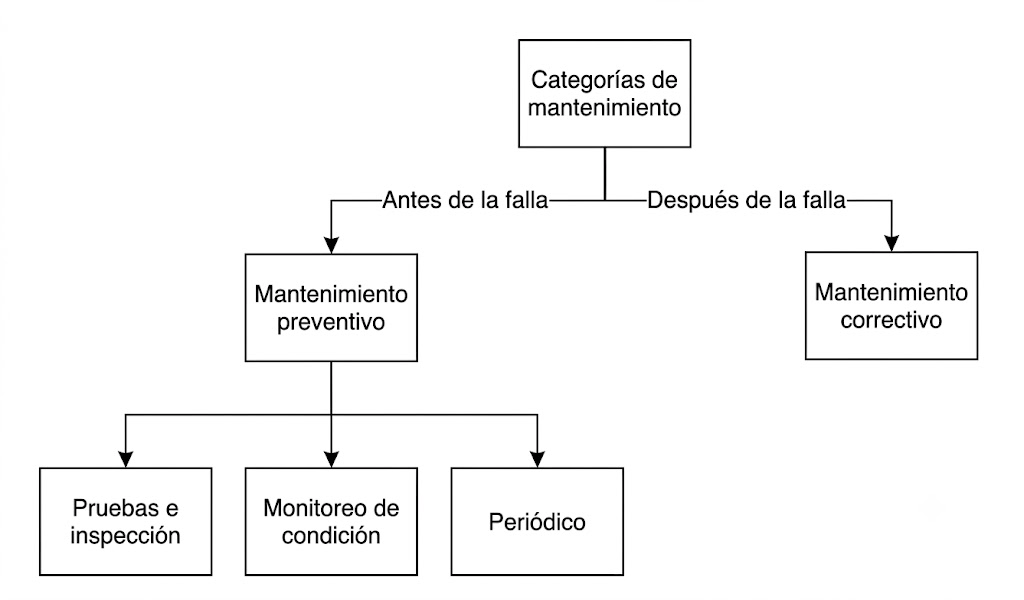
\includegraphics[width=0.8\textwidth]{assets/figures/theoretical_framework/img_maintenance_categories.png}
    \label{fig:maintenance_categories}

    \caption*{\textit{Nota}. \textnormal{Figura extraída de \textcite[p. 28]{ISO:2006}}}
    
\end{figure}
%\vspace{-1.6\baselineskip}

        \subsubsection{Mantenimiento correctivo}

            El mantenimiento correctivo, también denominado como mantenimiento básico, es la metodología de llevar a cabo actividades en el momento en el que las propiedades o activos de la empresa dejan de realizar el servicio para el que fueron diseñados, es decir cuando se da la detección del evento de falla \parencite{MEDRANO:2017}.

            Trabajar con el enfoque reactivo que implica esta metodología trae consigo la aparición de pérdidas debido a las paradas de producción, dado que la mano de obra se encontrará inactiva a la vez que se generan retrasos en el cumplimiento de los programas. \parencite{GALLARA:2020}.

        \subsubsection{Mantenimiento preventivo}\label{subsec:preventive_maintenance}

            El mantenimiento preventivo se define en base al periodo de tiempo previo a que ocurra la falla de un equipo, disminuyendo acciones correctivas que comprometen la disponibilidad de estos. Básicamente, el mantenimiento preventivo “consiste en programar inspecciones y revisiones a los equipos o máquinas, apoyándose en el conocimiento de estas en base a la experiencia de los ingenieros o técnicos, así también como el historial de la máquina” \parencite[p. 12]{TOLEDO:2018}.

            \paragraph{Enfoques del mantenimiento preventivo}

                La \textcite{IBM:SF} en su página web desglosa el mantenimiento preventivo en los siguientes cuatro tipos o enfoques para el planteamiento de rutinas o intervenciones:

                \begin{itemize}
                    
                    \item Mantenimiento preventivo según su uso.

                    \item Mantenimiento preventivo según plazo o calendario.

                    \item Mantenimiento predictivo.

                    \item Mantenimiento prescriptivo.

                \end{itemize}

    \subsection{La información en entornos de mantenimiento}

        La información se puede definir como el conjunto de datos que permiten conocer mejor el entorno de una empresa y con estos se disminuye la incertidumbre a la vez que se favorece la toma de decisiones acertadas, \textcite{LAPIEDRA:2021}. De acuerdo con \textcite{AENOR:2016}, el registro de datos generado tras la ejecución de actividades de mantenimiento constituye una herramienta de valor para el ingeniero de mantenimiento y el responsable de confiabilidad, particularmente en la estimación de la disponibilidad de los equipos. Entre los datos más relevantes que conviene registrar por cada máquina, se encuentran los listados en la Tabla \ref{tab:maintenance_data}.

        \input{assets/tables/tab_maintenance_data.tex}

        \subsubsection{Gestión de la información}

            \textcite{FONT:2014} describen que la gestión de Información abarca un conjunto de acciones dirigidas a recolectar información que cubra criterios de calidad, pertinencia, oportunidad y costo apropiados de acuerdo a las demandas del usuario; siendo fundamental el uso de las tecnologías de la información y las comunicaciones. Se tiene como objetivo ordenar y emplear la información, que provenga de fuentes tanto internas como externas, con el fin de simplificar su operación, aprendizaje y adaptación a los cambios del entorno.

        \subsubsection{Flujo de la información}

            Uno de los aspectos que incide directamente en la gestión de la información en entornos de mantenimiento es la estructura organizacional bajo la cual se concibe la empresa. La información manejada de forma centralizada tiene ventajas en su capacitación, manipulación y uso, además de disminuir las inconsistencias. Por su parte, “la descentralización permite adaptar las necesidades del usuario, por lo tanto, motiva al usuario, facilita el reparto de las tareas y multiplica la eficacia de las funciones directivas” \parencite[p. 3]{ARRIBAS:2000}. \textcite[p. 7]{BEN-DAYA:2009} señalan que en empresas de gran magnitud lo ideal es la estructura descentralizada, siendo la centralización lo recomendado para el caso de empresas de menor tamaño.

        \subsubsection{Tipos de información en mantenimiento}

            Complementario a los datos presentados en la Tabla \ref{tab:maintenance_data}, se presentan otras fuentes que respaldan y adicionan algunos puntos a considerar respecto al sistema de información de mantenimiento. Según la \textcite{COVENIN:1993} se describe a un sistema de información como “un conjunto de procedimientos interrelacionados, formales o informales, que permite la captura, procesamiento y flujo de información requerida en cada uno de los niveles de la organización” (p. 10), presentando procedimientos que contiene un sistema genérico de información de mantenimiento, los cuales contienen: codificación de los objetos de mantenimiento, registro de objetos de mantenimiento, instrucciones técnicas del mantenimiento, procedimiento de ejecución y programación del mantenimiento.
        
        \subsubsection{Gestión del conocimiento}

            En el contexto organizacional, el conocimiento representa uno de los activos más valiosos con los que cuenta una empresa, pues a diferencia de otros recursos, no se agota con su uso sino que se enriquece con la práctica y la experiencia acumulada. Su naturaleza es compleja y multidimensional, y como señalan \textcite{DAVENPORT:1998}, puede entenderse como una mezcla de experiencia enmarcada, valores, información contextual y visión experta que proporciona un marco para evaluar e incorporar nuevas experiencias e información; y que en las organizaciones no reside únicamente en documentos o repositorios, sino también en rutinas, procesos, prácticas y normas organizativas.

            El reconocer al conocimiento como un elemento vivo, distribuido y propio del recurso humano dentro de las organizaciones, es precisamente lo que genera la necesidad de gestionarlo de manera estratégica, dando lugar así al concepto de gestión del conocimiento. La gestión del conocimiento se define como “un enfoque y un conjunto de prácticas empresariales diseñadas para identificar, capturar, organizar, almacenar, compartir y aplicar el conocimiento dentro de una organización.” \parencite[p. 3]{RAMOS:2024}. Su alcance, sin embargo, va más allá de la simple administración de información, ya que implica la articulación de procesos, personas y tecnologías para favorecer la creación y el aprovechamiento del conocimiento. En este sentido, la gestión del conocimiento puede entenderse como un proceso que integra el tratamiento de datos e información mediante las tecnologías de la información con las capacidades humanas de creatividad, innovación, trabajo colaborativo y construcción de una visión compartida \parencite{MALHOTRA:2005}.

        \subsubsection{Sistema de gestión de conocimiento}

            Según el \textcite[p. 6]{ICONTEC:2019} se dan pautas para desarrollar un sistema eficaz de gestión del conocimiento con el cual las empresas perciban una nueva fuente de generación de valor. Dentro de los puntos de la generación del conocimiento aparece la retención del conocimiento, definida como la capacidad de salvaguardar a la organización contra la pérdida de conocimiento. Asimismo se hacen anotaciones respecto a la protección del conocimiento en relación a las posibles rotaciones o variaciones del personal, además de tener la información documentada y respaldada.

            También se hace énfasis en la necesidad de incluir actividades y comportamientos para la transferencia de conocimientos listando cuatro ítems, siendo uno de ellos denominado la combinación donde se busca “sintetizar, conservar, formalizar, estructurar o clasificar el conocimiento codificado, haciendo que este sea accesible y fácil de encontrar” \parencite[p. 7]{ICONTEC:2019}. Con lo anterior, se identifican puntos de convergencia entre la gestión del conocimiento en mantenimiento y el planteamiento de soluciones tecnológicas como la realidad aumentada, reconociendo el papel de las tecnologías como apoyo a dicha gestión.

    \subsection{Modelos 3D y su integración con la realidad aumentada}

        El modelado 3D constituye una base fundamental para el desarrollo de experiencias de realidad aumentada. Se trata de una representación tridimensional de un objeto mediante software especializado cuyo proceso incia desde la adquisición de datos y culmina con un modelo virtual visualmente interactivo a través de una computadora, \parencite{GHUGE:2023}.

        La importancia de los modelos 3D radica en su capacidad para enriquecer la interacción y la inmersión dentro de entornos virtuales y aumentados. En este sentido, \textcite{GHUGE:2023} señala que los objetos 3D son cruciales para la creación de experiencias inmersivas en aplicaciones como el turismo virtual, las simulaciones de entrenamiento y la narración interactiva. Dado que estos modelos suelen emplearse como elementos digitales superpuestos al entorno real, resulta necesario comprender el concepto de realidad aumentada. Bajo esta perspectiva, \textcite{ARENAS:2022} describe la realidad aumentada como una tecnología capaz de complementar el entorno físico del usuario mediante la incorporación, en tiempo real, de información digital superpuesta.

        \subsubsection{Representación geométrica}

            La geometría de un objeto puede describirse mediante dos grandes tipos de representación: implícita y explícita. Dentro de las representaciones explícitas se distinguen, a su vez, las paramétricas y las no paramétricas. Las primeras abarcan tanto formas primitivas como líneas, círculos, planos, esferas, cilindros o figuras cuadráticas como formas más complejas, entre las que se encuentran las curvas de Bezier, B-splines y NURBS \parencite{PATRAUCEAN:2015}. Las representaciones no paramétricas, por su parte, se emplean en casos donde las formas paramétricas resultan insuficientes, siendo ejemplos característicos las nubes de puntos y las mallas polinomiales \parencite{PATRAUCEAN:2015, FOUGEROLLE:2005}.

        \subsubsection{Herramientas para modelado 3D}

            Los modelos paramétricos se crean a partir de un software especializado, que brinda herramientas de diseño paramétricas y técnicas de modelado procedural que permiten a los diseñadores la definición de parámetros, reglas y algoritmos \textcite{GHUGE:2023}. Algunas de las alternativas más populares en el mercado de diseño paramétrico son:

            \begin{itemize}

                \item AutoCAD, por Autodesk.
                
                \item Solid Edge, por Siemens.
                
                \item SOLIDWORKS, por Dassault Syst\`emes.
                
                \item Fusion 360, por Autodesk.
                
                \item Onshape, por PTC.
                
                \item Inventor, por Autodesk.
                
                \item FreeCAD, como alternativa gratuita y de código abierto.
                
            \end{itemize}

        \subsubsection{Formatos de modelos 3D para su uso en realidad aumentada}

            Para un uso eficiente de los recursos que ofrece un dispositivo móvil tales como: Smartphones, Tablets, o visores de realidad mixta; es necesario el uso de un formato basado en mallas (Mesh), la cual tal como dice \parencite{GHUGE:2023}, es una colección de vértices, ejes y caras, que definen la forma del objeto 3D, donde se incluyen diferentes tipos de mallas tales como: mallas polinomiales, NURBS (Non-Uniform Rational B-Splines) y superficies de subdivisión.

            En el contexto de una aplicación de realidad aumentada, la carga dinámica de modelos resulta indispensable para permitir al usuario interactuar con los objetos del entorno, ya sea cargándolos, seleccionándolos o eliminándolos en tiempo real. Para ello, formatos como .glTF (Graphics Library Transmission Format) y su variante binaria .glb ofrecen una solución eficiente, al estructurar los modelos en una jerarquía de nodos, clasificados en nodos padre e hijos, que pueden representar objetos como mallas, máscaras y cámaras. A su vez, estas mallas pueden referenciar materiales asociados a texturas e imágenes. Para la exportación de modelos en estos formatos, incluyendo animaciones por fotogramas clave que permiten la locomoción procedural de partes, se destacan las siguientes alternativas:

            \begin{itemize}

                \item El uso de las características de realidad extendida de SolidWorks, que se incluyen a partir de la versión estándar 2019, donde se pueden transformar las animaciones de estudios de movimiento en secuencias de fotogramas clave glTF.
                
                \item El uso del software de modelado Blender, el cual trabaja directamente con secuencias de fotogramas y tiene como posibilidad la exportación de estas en formato glTF, como alternativa gratuita y de código abierto.
                
            \end{itemize}

        \subsubsection{Tipos de realidad aumentada}

            La realidad aumentada es agrupada en dos categorías basadas por su funcionalidad al momento de su activación, una categoría define la inicialización por medio de activadores y la otra es basada en la visualización o contexto del entorno \parencite{STEWART:2016}. Estas categorías poseen diferentes tipos o métodos de activación sintetizados en la Tabla \ref{tab:augmented_reality_types}.

            \input{assets/tables/tab_augmented_reality_types.tex}